\documentclass{article}
\usepackage{graphicx}
\title{\textbf{homework-01}}
\author{our group name here}
\date{\today}

\begin{document}
\maketitle

\section{Broken Chessboard and Jumping With Coins}
\subsection{Tiling a Damaged Checkerboard}

\begin{flushleft}
\textbf{Exercise 1.1.} \\
Firstly, we color the chessboard in black and white.\\
\begin{center}
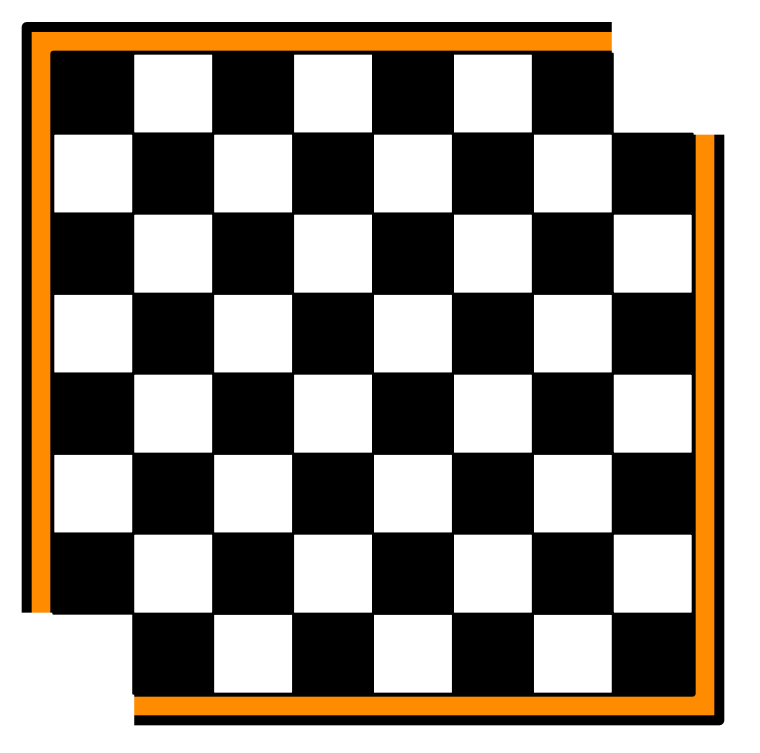
\includegraphics[scale=0.3]{1_1_1.png}
\end{center}
So now, we have 32 black squares and 30 white squares.\\
And if we put a tile in this chessboard, it will cover exactly a black square and a white squre, no matter how we put it.\\
So if we continue put tiles on it, we will have two black squares left in the end.\\
\begin{center}
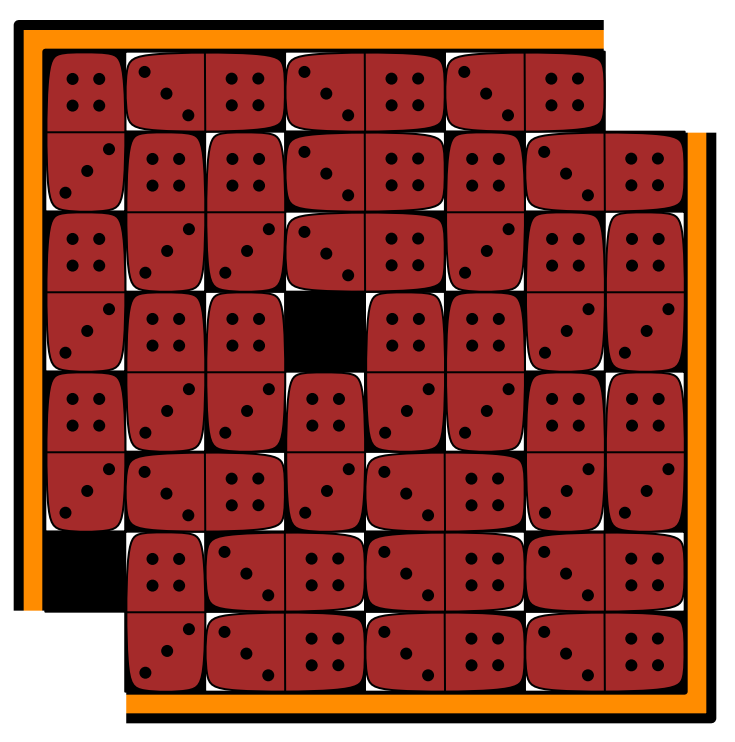
\includegraphics[scale=0.3]{1_1_2.png}
\end{center}
It means that whatever we do we will always get stuck because there are always two more black squares than white squares.\\
So it is obvious that we cannot tile this damaged chessboard.\\

\textbf{Exercise 1.2.} \\
...

\end{flushleft}
\subsection{Jumping with Coins}

\begin{flushleft}
\textbf{Exercise 1.3.} \\
...

\textbf{Exercise 1.4.} \\
...

\textbf{Exercise 1.5.} \\
A coin is at a position $(x,y)\in\mathbf{R}^2$ .\\
we assume that in the begning the pos are (0,0),(0,1),(1,0),(1,1).\\


\textbf{Exercise 1.6.} \\
...

\textbf{Exercise 1.7.} \\
...

\textbf{Exercise 1.8.} \\
...

\end{flushleft}
\section{Exclusion-Inclusion}
\subsection{Sets}

\begin{flushleft}
\textbf{Exercise 2.1.} \\
...

\textbf{Exercise 2.2.} \\
...

\textbf{Exercise 2.3.} \\
...

\end{flushleft}
\section{Feasible Intersection Patterns}

\begin{flushleft}
\textbf{Exercise 3.1.} \\
...

\textbf{Exercise 3.2.} \\
...

\textbf{Exercise 3.3.} \\
...
\end{flushleft}
\end{document}